\chapter{Transformer}
\label{chap:4}

本章目标在于说明 Transformer 的概念,同时说名在其 Transformer 的文献上的工作进行说明与复现工作。本作业其专案为 kancheng/kan-cs-report-in-2021 ,程式码则可于 kan-cs-report-in-2021/AI/pytorch-transformer 中找到,实验设备为 MacBook Pro (Retina, 15-inch, Mid 2014) 和 Acer Aspire R7 与 Google Colab。

\section{Transformer 理解}

此节目标在于说明 Transformer 概念理解,根据原本的技术文件与论文的内容进行说明和理解进行整理。其内容包含了原本论文的该概念描述,同时也对实际原理进行说明。

\begin{figure}[htb]
\centering 
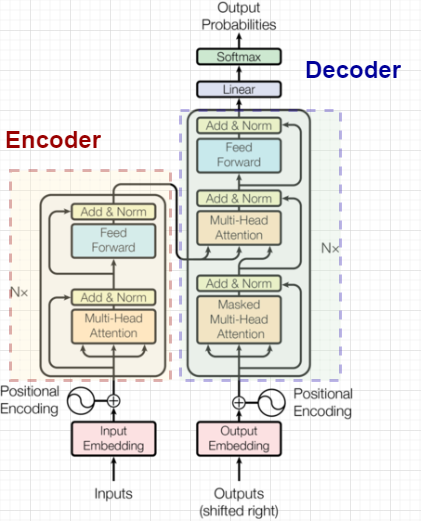
\includegraphics[width=0.5\textwidth]{img/c4s1.png} 
\caption{直观架构}
\label{Test}
\end{figure}

\subsection{原理简述}

单纯从 Google 於 2017 所發表的 Attention is All You Need 中的 Transformer,其架构 直观来看可以分为  Encoder 和 Decoder 两大部分。就与过往的传统 RNN、CNN 模型不同在于,工作是由 Attention 机制来进行实现,而且由于 Encoder 端是并行计算,具有训练时间缩短的优势。

在此简述其模型的优势,从过往的研究来看,传统 seq2seq 最大的问题在于该模型会将 Encoder 端的所有信息压缩到一个固定长度的向量里面,同时将其作为 Decoder 端首个隐藏状态的输入,来预测 Decoder 端第一个单词 token 的隐藏状态。当输入序列比较长的时候,此方法很会损失 Encoder 端那方的很多信息,而且将大量的把该固定向量送入 Decoder 端,Decoder端那方很有可能不能够关注到其想要我们想要关注的信息。同时模型计算不可并行,其计算隐层状态 $h_t$ 依赖于 $h_{t-1}$ 以及状态 $t$ 时刻的输入,因此需要耗费大量时间。而 Transformer 优点则是在于 Transformer 架构完全依赖于 Attention 机制,解决了输入输出的长期依赖问题,同时拥有并行计算的能力,大大减少了计算资源的消耗。self-attention 模块则会让源序列和目标序列首先 “自关联” 起来,在此情况下源序列和目标序列自身的 embedding 表示所蕴含的信息会更加丰富,而且后续的 FFN 层也增强了模型的表达能力。而 Muti-Head Attention 模块使得 Encoder 端拥有并行计算的能力

%\subsection{seq2seq}

\section{Transformer 研究}

本节目标示根据近期研究进行追溯,该节先是对 Transformers in vision: A survey \cite{khan2021transformers} 进行概括,同时找出六篇研究进行工作调研与总结并进行整理,所以该节使用文献如下条列 :

\begin{itemize}
\item Transformers in Vision: A Survey
\item Set Transformer: A Framework for Attention-based Permutation-Invariant Neural Networks
\item Deep amortized clustering
\item Non-local Neural Networks
\item Axial-DeepLab: Stand-Alone Axial-Attention for Panoptic Segmentation
\item Taming Transformers for High-Resolution Image Synthesis
\item Video Action Transformer Network
\end{itemize}


\subsection{工作追溯}

Transformers in vision: A survey 该篇为视觉中的 Transformer 和自注意力综述涵盖了 transformer 在视觉领域的广泛应用,包括如图像分类,目标检测,动作识别和分割等流行的识别任务,生成模型,如视觉问题解答和视觉推理等多模式任务,又如活动识别,视频预测等视频处理,再如图像超分辨率和彩色化 的 low-level 视觉和点云分类和分割等 3D 分析。

该篇研究先说明 Transformer 模型与研究的重要性,并说明  Transformer 在自然语言任务中获得惊人结果,并引起了计算机视觉领域的兴趣跟注意得原因,研究它们在计算机视觉问题中的应用,Transformer 与类似如长短期记忆 (LSTM)等的循环网络相比,Transformers 的显着优势之一是能够对输入序列元素之间的长期依赖关系进行建模,并支持序列的并行处理。 Transformer 与卷积网络不同,Transformer 的设计需要最小的归纳偏差,自然适合作为集合函数。此外 Transformers 的简单设计允许使用类似的处理块处理多种模态(例如,图像、视频、文本和语音),并展示了对超大容量网络和庞大数据集的出色可扩展性。这些优势使使用 Transformer 网络的许多视觉任务取得了令人兴奋的进展。本次调查旨在全面概述计算机视觉学科中的 Transformer 模型。研究者首先介绍 Transformers 成功背后的基本概念,即自我注意、大规模预训练和双向特征编码。然后,我们介绍了转换器在视觉中的广泛应用,包括如图像分类、对象检测、动作识别和分割等流行的识别任务领域,生成建模领域,又如视觉问答、视觉推理和视觉基础等多模态任务,再如活动识别、视频预测的视频处理领域,或者是图像超分辨率、图像增强和着色的 low-level vision 领域和点云分类和分割的 3D 分析。研究者比较了流行技术在架构设计和实验价值方面的各自优势和局限性。最后该研究对开放的研究方向和未来可能的工作进行了分析,此研究希望这项努力将进一步激发社区的兴趣,以解决当前在计算机视觉中应用变压器模型所面临的挑战。最后将该篇研究的整理用简略的条例表示如下:
\begin{itemize}
\item [1.] 用于图像识别的 Transformer

\begin{itemize}
\item Non-local Neural Networks
\item Criss-cross Attention
\item Stand-alone Self-Attention
\item Local Relation Networks
\item Attention Augmented Convolutional Networks
\item Vectorized Self-Attention
\item Vision Transformer
\item Data-efficient Image Transformers
\end{itemize}


\item [2.] 用于目标检测的 Transformer

\begin{itemize}
\item DETR
\item Deformable - DETR
\end{itemize}


\item [3.] 用于分割的 Transformer

\begin{itemize}
\item Axial-attention for Panoptic Segmentation
\end{itemize}


\item [4.] 用于图像生成的 Transformer

\begin{itemize}
\item Image GPT
\item Image Transformer
\item High-resolution Image Synthesis
\item SceneFormer
\end{itemize}


\item [5.] 用于 low-level 视觉的 Transformer

\begin{itemize}
\item Transformers for super-resolution
\item Transformers for Image Enhancement Tasks
\item Colorization Transformer
\end{itemize}


\item [6.] 用于多模态任务的 Transformer

\begin{itemize}
\item ViLBERT: Vision and Language BERT
\item LXMERT
\item VisualBERT
\item VL-BERT
\item Unicoder-VL
\item UNITER
\item Oscar: Object-Semantics Aligned Pre-training
\item Vokenization
\item Vision-and-Language Navigation
\end{itemize}


\item [7.] 用于视频理解的 Transformer

\begin{itemize}
\item VideoBERT: Joint Video and Language Modeling
\item Parameter Efficient Multi-modal Transformers
\item Video Action Transformer
\item Skeleton-based Action Recognition
\end{itemize}


\item [8.] 用于 Low-shot 学习的 Transformer

\begin{itemize}
\item Cross-transformer
\item FEAT: Few-shot Embedding Adaptation
\end{itemize}


\item [9.] 用于聚类的 Transformer
 
\begin{itemize}
\item Set Transformers 
\end{itemize}


\item [10.] 用于 3D 分析的 Transformer
 
\begin{itemize}
\item Point Transformer
\item Point-cloud Transformer
\item Pose and Mesh Reconstruction
\end{itemize}

\end{itemize}

\begin{figure}[htb]
\centering 
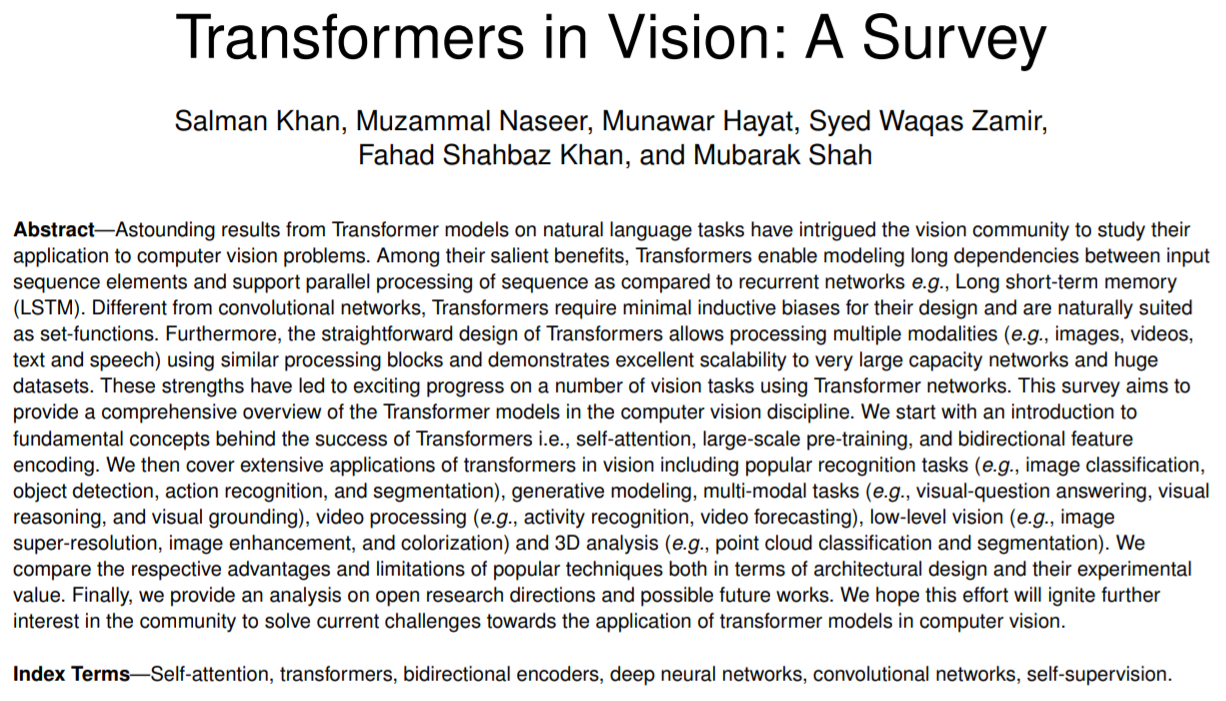
\includegraphics[width=0.7\textwidth]{img/c4y1.png} 
\caption{Transformers in vision: A survey}
\label{Test}
\end{figure}

\subsection{Set Transformer: A Framework for Attention-based Permutation-Invariant Neural Networks}

其原因在于许多机器学习任务,例如多实例学习、3D 形状识别和小样本图像分类,都是在实例集上定义的,而由于此类问题的解决方案不依赖于集合元素的顺序,用于解决这些问题的模型应该是置换不变,所以该研究提出了一个基于注意力的神经网络模块,即 Set Transformer,专门设计用于对输入集中元素之间的交互进行建模。提出的模型由一个编码器和一个译码器组成,两者都依赖于注意力机制,而为了降低计算复杂度,研究者引入了一种注意力机制,其灵感来自于从稀疏高斯过程文献中引入点方法。它将自注意力的计算时间从集合中元素的数量的二次减少到线性。该研究表明的模型在理论上具有吸引力,并且在一系列任务上对其进行了评估,与最近的集合结构数据方法相比,表现出更高的性能。

该研究说明学习表征已被证明是深度学习及其许多成功案例的基本问题,而深度学习解决的大多数问题都是基于实例的,并采用将固定维输入张量映像到其相应目标值的形式 (Krizhevsky et al., 2012; Graves et al., 2013),而对于某些应用程序,研究者认为会需要处理集合结构化数据。再此研究者说明多实例学习 (Dietterich et al., 1997; Maron \& Lozano-Perez , 1998) 是这种集合输入问题的一个例子,其中给定一组实例作为输入,相应的目标是整套。
其他问题,例如 3D 形状识别 (Wu et al.,2015; Shi et al., 2015; Su et al., 2015; Charles et al., 2017) 、序列排序 (Vinyals et al., 2016) 以及各种 集合操作(Muandet et al., 2012; Oliva et al., 2013; Edwards \& Storkey, 2017; Zaheer et al., 2017)也可以被视为集合输入问题,同时许多元学习 (Thrun \& Pratt, 1998; Schmidhuber, 1987) 问题使用不同但相关的任务进行学习,也可以视为 setinput 任务,其中输入集对应于单个任务的训练数据集。

例如少样本图像分类 (Finn et al., 2017; Snell et al., 2017; Lee \& Choi, 2018) 通过使用一组支持图像构建分类器来运行,而该分类器使用查询图像进行评估,集合输入问题的模型应该满足两个关键要求。首先第一个要求在于,它应该是排列不变的——模型的输出在输入集中元素的任何排列下都不应该改变,其次此类模型应该能够处理任何大小的输入集。虽然这些要求源于集合的定义,但它们在基于神经网络的模型中并不容易满足:经典的前馈神经网络违反了这两个要求,并且 RNN 对输入顺序很敏感,而近来 Edwards \& Storkey (2017) and Zaheer et al. (2017)  提出了满足这两个标准的神经网络架构,我们称之为集合池方法,在此模型中在集合中的每个元素首先被独立地馈送到接受固定大小输入的前馈神经网络。然后使用池化操作 (均值(mean), 总和(sum), 最大值(max) or 类似(similar)).聚合得到的特征空间嵌入,而通过对聚合嵌入的进一步非线性处理获得最终输出。
这种非常简单的架构满足上述两个要求,更重要的是它被证明是任何集合函数的通用逼近器 (Zaheer et al., 2017)。由于此类特性可以根据黑盒方式学习输入集与其目标输出之间的复杂映像,就像前馈或循环神经网络一样,尽管这种集合池方法在理论上很有吸引力,但研究者仍不清楚我们是否可以仅使用基于实例的特征提取器和简单的池操作来很好地近似复杂的映射。
由于集合中的每个元素都在集合池操作中独立处理,因此必须丢弃一些有关元素之间交互的信息,这可能会使一些问题不必要地难以解决。考虑摊销聚类的问题,研究者会想学习从输入点集到该集内点簇中心的参数映射,即使面对于二维空间中的玩具数据集,这也不是一个容易的问题。

主要的困难在于参数映像必须在对解释模式进行建模时将每个点分配给其相应的集群,这样得到的集群就不会试图解释输入集的重迭子集。由于这种先天的困难,聚类通常通过迭代算法来解决,这些算法细化随机初始化的聚类直到收敛。
尽管具有集合极化操作的神经网络可以通过学习量化空间来近似这种摊销映射,但一个关键的缺点是这种量化不能依赖于集合的内容。
这限制了解决方案的质量,也可能使此类模型的优化更加困难;研究者在该研究名为 Experiments 的第 5 节,让我们知道经验表明,此类池化架构存在欠拟合的问题。
该研究提出了一种称为 Set Transformer 的新型集输入深度神经网络架构(cf. Transformer, (Vaswani et al., 2017))。 而 Set Transformer 的新颖之处在于三个重要的设计选择:

\begin{itemize}
\item 研究使用自注意力机制来处理输入集中的每个元素,这允许我们的方法自然地编码集中元素之间的成对或高阶交互。
\item 研究提出了一种将完全自注意力 (e.g. the Transformer) 的 $O(n^{2})$ 计算时间减少到 $O(nm)$ 的方法,其中 m 是固定的超参数,允许该研究的方法扩展到大型输入集。
\item 研究使用自注意力机制来聚合特征,这在问题需要多个相互依赖的输出时特别有用,例如元聚类问题 (the problem of meta-clustering),其中每个聚类中心的含义在很大程度上取决于其相对位置到其他集群。
\end{itemize}

该研究将 Set Transformer 应用于几个集合输入问题,并凭经验证明了这些设计选择的重要性和有效性,并表明我们可以为大多数任务实现最先进的性能。

\subsection{Deep amortized clustering}

研究者们提出了一种深度摊销聚类 (DAC; deep amortized clustering),这是一种神经架构,它学习使用一些前向传播有效地对数据集进行聚类,其 DAC 隐式地学习是什么构成了一个集群,如何将数据点分组到集群中,以及如何计算数据集中的集群数量。而 DAC 是使用标记数据集进行元学习的,这一过程不同于传统的聚类算法,而传统聚类算法通常需要手工指定的关于聚类形状和结构的先验知识。研究者凭经验表明,在合成数据和图像数据上,DAC 可以有效且准确地对来自用于生成训练数据集的相同分布的新数据集进行聚类。

而从图可知,该研究的模型每次迭代识别一个集群(顶部),使其能够找到任意数量的集群(底部),其聚类是无监督机器学习中的一项基本任务,用于将相似的数据点分组到多个集群中。除了在许多下游任务中的有用性之外,聚类是可视化和理解数据集底层结构的重要工具,也是认知科学中的分类模型,而大多数聚类算法有两个基本组成部分——如何定义集群以及如何将数据点分配给这些集群。

前者通常使用度量来测量数据点之间的距离,或使用描述集群形状的生成模型来定义,而后者如何将数据点分配给集群,然后通常会迭代优化 w.r.t. 基于集群定义导出的目标函数。
请注意聚类定义是用户定义的,是用户对聚类过程的先验知识的反映,不同的定义导致不同的聚类,然而实践中使用的集群定义通常非常简单,例如 k-means 中的集群是根据到质心的 2 距离定义的,而高斯是混合模型中集群的常用生成模型。近来深度学习的进步促进了以黑盒方式逼近复杂函数,本研究中与聚类问题相关的一个特殊应用是摊销推理 (Gershman \& Goodman, 2014; Stuhlmüller et al., 2013),其中训练神经网络以预测潜在变量的状态模型或概率程序。而在学习集输入神经网络的背景下 (Zaheer et al., 2017),Lee et al. (2019)  表明可以分摊高斯混合 (MOG;a Mixture of Gaussians) 的迭代聚类过程,而 Pakman et al. (2019) 证明可以训练神经网络将数据点顺序分配给集群。此两种方法都可以解释为使用神经网络对给定数据集的集群分配和参数进行摊销推理,而在此要注意的部分在于,一旦将神经网络用于摊销聚类,研究者们就可以利用它们的灵活性来使用更复杂的方法来定义聚类。此外,摊销网络可以使用生成的数据集进行训练,其中地面实况聚类是已知的。这也可以解释为隐式学习训练数据集底层的集群定义,这样摊销推理(大约)会产生适当的集群。

从某种意义上来看,这与神经过程 (Garnelo et al., 2018b;a)有着相似的哲学,后者从多个数据集进行元学习 (meta-learns) 以学习函数的先验,回到该研究来看,研究者以这些先前的工作为基础,并提出了深度摊销聚类 (DAC;Deep Amortized Clustering),该研究与之前的工作一样,DAC 中的摊销网络使用生成的数据集进行训练,其中地面实况聚类是已知的,像 Lee et al. (2019),DAC 使用 Set Transformer,但与 Lee et al. (2019) 因为它按顺序生成集群,这可以根据数据集的复杂性生成不同数量的集群。此研究的方法还扩展了 Lee et al. (2019) 从 MOG 到更复杂的集群定义问题,可以说这些问题更难手动指定,更容易从数据中进行元学习,而其工作也不同于 Pakman et al.(2019),因为我们的网络并行处理数据点,而 Pakman et al. (2019)按顺序处理它们,这可以说是可扩展性较低,并且限制了对较小数据集的适用性。

该研究的组织如下。研究者们首先在该研究的名为 A PRIMER ON SET TRANSFORMER AND AMORTIZED CLUSTERING 的第 2 节中,去描述在整篇论文中使用的置换不变集变换器模块。,同时在名为 DEEP AMORTIZED CLUSTERING 的第 3 节中,此研究描述了研究者们如何实现一次识别一个集群的核心思想,并描述了研究者的聚类框架 DAC 在复杂数据集上解决 DAC 有几个挑战,同时按难度顺序构建此论文 。

\begin{figure}[htb]
\centering 
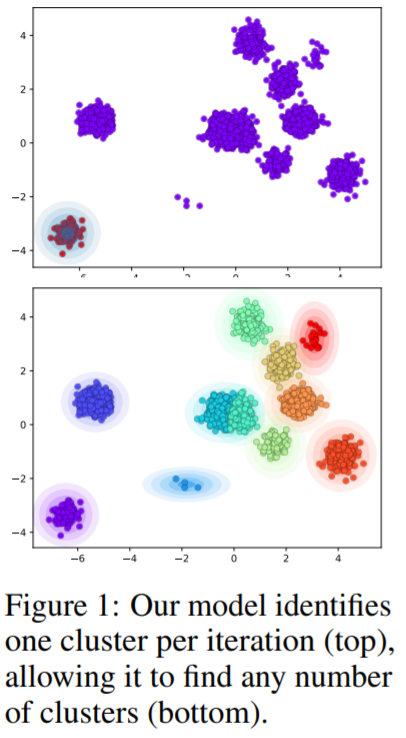
\includegraphics[width=0.3\textwidth]{img/pa2.png} 
\caption{Deep amortized clustering}
\label{Test}
\end{figure}


\subsection{Non-local Neural Networks}

此研究指出卷积和循环操作都是一次处理一个局部邻域的构建块。在该研究中,研究者们将非本地操作呈现为用于捕获远程依赖项的通用构建块系列,而受计算器视觉中经典的非局部均值方法的启发,研究者的非局部操作将某个位置的响应计算为所有位置特征的加权和,而此构建块可以插入到许多计算器视觉架构中。同时在视频分类任务上,即使没有任何繁杂的东西,研究者的非本地模型也可以在 Kinetics 和 Charades 数据集上与当前的竞争者竞争或胜出,另外在静态图像识别中,研究者们的非局部模型改进了 COCO 任务套件上的对象检测/分割和姿态估计,可捕获远程依赖关系在深度神经网络中至关重要。对于如在语音(speech)、语言(language) 的循环操作(recurrent operations) 与序列数据(sequential data) 是远程依赖建模的主要解决方案,而对于图像数据来说,长距离依赖是由卷积运算的深堆栈形成的大感受野建模。另外卷积运算和循环运算都在空间或时间上处理局部邻域, 因此只有在重复应用这些操作时才能捕获远程依赖关系,通过数据逐步传播信号。在此重复本地操作有几个限制,首先它在计算上效率低下,其次它会导致需要仔细解决的优化困难。

最后这些挑战使得多跳依赖建模变得困难,比如当需要在远距离位置之间来回传递消息的时候。在该研究中,研究者将非本地操作作为一种高效、简单且通用的组件,用于捕获深度神经网络的远程依赖关系,当中所提出的非局部操作是计算器视觉中经典非局部平均操作的推广。直观地说,非局部操作将某个位置的响应计算为输入特征图中所有位置的特征的加权。此组位置可以是空间、时间或时空,这意味着我们的操作适用于图像、序列和视频问题。使用非本地操作有几个优点:(a) 与循环和卷积运算的渐进行为相反,非局部运算通过计算任意两个位置之间的相互作用直接捕获远程依赖关系,而不管它们的位置距离如何;(b) 正如我们在实验中所展示的,即使只有几层,非本地操作也是有效的,并且可以达到最佳效果;(c) 最后,研究非本地操作保持了可变的输入大小,并且可以很容易地与其他操作,例如研究者将使用的卷积结合起来,同时研究展示了非本地操作在视频分类应用中的有效性,而在视频中远距离的空间和时间像素之间会发生远程交互。

作为该研究的基本单元的单个非本地块可以前馈方式直接捕获这些时空依赖性,有了一些非局部块,研究者认为非局部神经网络且包含包括膨胀变体的架构对于视频分模拟 2D 和 3D 卷积网络更为准确。此外,非局部神经网络比 3D 卷积神经网络在计算上更经济,同时在 Kinetics 和 Charades 数据集上介绍了综合消融研究。仅使用 RGB 而没有任何类似光流、多尺度测试复杂的东西,本研究的方法在两个数据集上取得的结果与最新的比赛获胜者相当或更好。为了证明非局部操作的普遍性,研究进一步介绍了 COCO 数据集上的对象检测/分割和姿态估计实验,而在强大的 Mask R-CNN 基线 之上,研究者的非局部块可以以很小的额外计算成本提高所有三个任务的准确性,连同视频中的证据,这些图像实验表明非局部操作通常是有用的,并且可以成为设计深度神经网络的基本构建块。从图中我们可以看到网络中的一个时空非局部操作训练用于 Kinetics 中的视频分类,位置 $x_{i}$ 的响应由所有位置 $x_{j}$ 的特征的加权平均值计算,而此处仅显示最高权重的特征,在这个由我们的模型计算的示例中,请注意它如何将第一帧中的球与最后两帧中的球相关联。

\begin{figure}[htb]
\centering 
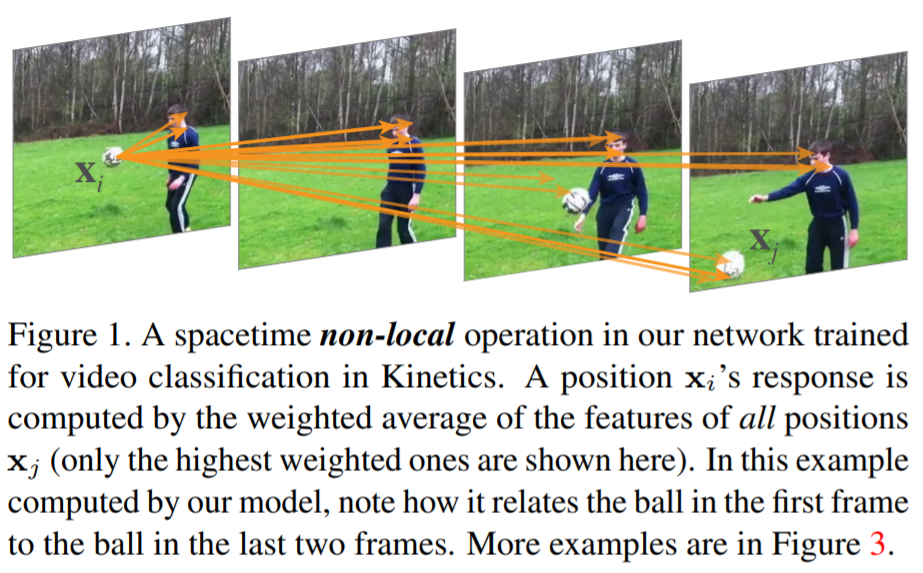
\includegraphics[width=0.7\textwidth]{img/pa3.png} 
\caption{Non-local Neural Networks}
\label{Test}
\end{figure}

\subsection{Axial-DeepLab: Stand-Alone Axial-Attention for Panoptic Segmentation}

卷积利用局部性来提高效率,代价是丢失了远程上下文,已采用自注意力来增强具有非本地交互作用的 CNN,最近的工作证明可以通过将注意力限制在局部区域来堆栈自注意力层以获得完全注意力网络,该研究试图通过将 2D 自注意力分解为两个一维自注意力来消除此约束,在此降低了计算复杂度,并允许在更大甚至全局区域内执行注意力。同时研究者还提出了一种位置敏感的自注意力设计,将两者结合产生研究者想要的位置敏感轴向注意层,这是一种新颖的构建块,可以堆栈以形成用于图像分类和密集预测的轴向注意模型。该研究证明了研究者的模型在四个大规模数据集上的有效性,特别在于其模型优于 ImageNet 上所有现有的独立自注意力模型,而研究者的 Axial-DeepLab 在 COCO 测试开发上比自下而上的最新技术提高了 2.8\% 的 PQ,先前的最新技术是通过我们的小变体实现的,该变体的参数效率为 3.8 倍,计算效率为 27 倍,Axial-DeepLab 还在 Mapillary Vistas 和 Cityscapes 上取得了最先进的结果。

卷积是计算器视觉的核心构建块,早期算法使用卷积滤波器来模糊图像、提取边缘或检测特征。前者与全连接模型相比,由于其效率和泛化能力,它在现代神经网络中得到了大量利用。卷积的成功主要来自平移等方差性和局部性的两个特性,平移等方差虽然不精确,但与成像的性质非常吻合,因此可以将模型推广到不同的位置或不同尺寸的图像。另一方面,局部性减少了参数计数和 M-Adds,然而它使建模远程关系具有挑战性,另外大量文献讨论了在卷积神经网络 (CNN) 中对远程交互进行建模的方法,而一些采用多孔卷积、更大的内核或图像金字塔,要么是手工设计的,又或者是通过算法搜索,另一行作品采用注意力机制,注意显示了它在语言建模、语音识别和神经字幕中对远程交互进行建模的能力。此后注意力已扩展到视觉,显著提升了图像分类、对象检测、语义分割、视频分类和对抗性防御。这些工作通过非局部或远程注意力模块丰富了 CNN,近来有研究已经提出将注意力层堆栈为没有任何空间卷积的独立模型并显示出有希望的结果,同时朴素的注意力在计算上是昂贵的,尤其是在大输入上。 提出的将局部约束应用于注意力,可以降低成本并能够构建完全注意力模型。同时局部约束限制了模型感受野,这对于分割等任务至关重要,尤其是在高分辨率输入上。在此项工作中,我们建议采用轴向注意力,它不仅可以进行高效计算,而且可以恢复独立注意力模型中的感受。

核心思想是将 2D 注意力分解为沿高度和宽度轴顺序的两个 1D 注意力,其效率使我们能够参与大区域并构建模型来学习远程甚至全局交互。此外,大多数先前的注意力模块不利用位置信息,这会降低如多尺度的形状或对象的注意力在建模与位置相关的交互中的能力。最近的作品会将位置术语引入注意力,但是以一种与上下文无关的方式。在该研究中,研究者将位置项增加为上下文相关,使研究的注意力对位置敏感,并具有边际成本。研究展示该研究的轴向注意力模型在 ImageNet 上进行分类的有效性,以及在三个数据集(COCO 、Mapillary Vistas 和 Cityscapes )上进行全景分割、实例分割、和语义分割。特别是,在 ImageNet 上,研究者通过用其位置敏感的轴向注意层替换所有残差块中的 3 × 3 卷积来构建 Axial-ResNet,并通过采用轴向注意层进一步使其获得完全注意。
因此该研究的 Axial-ResNet 在 ImageNet 上的独立注意力模型中取得了最先进的结果。而对于分割任务,研究者通过替换 Panoptic-DeepLab 中的主干将 Axial-ResNet 转换为 Axial-DeepLab。

在 COCO 上,研究者的 Axial-DeepLab 在测试开发集上以 2.8\% 的 PQ 优于当前自下而上的最新技术 Panoptic-DeepLab,而研究者还在 Mapillary Vistas 和 Cityscapes 上展示了最先进的分割结果。

总而言之,研究者的贡献有四方面:

\begin{itemize}
\item 所提出的方法是首次尝试构建具有大或全局感受野的独立注意力模型。
\item 该研究提出了位置敏感的注意力层,它可以更好地利用位置信息而不会增加太多的计算成本。
\item 该研究表明轴向注意力运作良好,不仅作为图像分类的独立模型,而且作为全景分割、实例分割和分割分割的支柱
\item 该研究的 Axial-DeepLab 在 COCO 上比自下而上的最新技术显著改进,实现了与两阶段方法相当的性能。
\end{itemize}

最后此研究还在 Mapillary Vistas 和 Cityscapes 上超越了之前最先进的方法。


\subsection{Taming Transformers for High-Resolution Image Synthesis}

研究首先指出在学习序列数据上的远程交互,transformers 继续在各种任务上显示出最先进的结果,而前者与 CNN 相比,它们不包含优先考虑局部交互的归纳偏差。这使它们具有表现力,但对于如高分辨率图像的长序列,在其计算上也不可行。

本研究展示瞭如何将 CNN 的归纳偏置的有效性与 Transformer 的表达能力相结合,使它们能够建模并从而合成高分辨率图像,大致分为 (i) 使用 CNN 来学习图像成分的上下文丰富的词汇,并反过来 (ii) 利用转换器在高分辨率图像中有效地对其组成进行建模。

该研究的方法很容易应用于条件合成任务,其中如对像类等非空间信息和如分割等空间信息都可以控制生成的图像,特别在于此研究展示了带有转换器的百万像素图像的语义引导合成的第一个结果,并在类条件 ImageNet 上的自回归模型中获得了最先进的技术。

Transformer 正在兴起——它们现在是语言任务的事实上的标准架构,并且越来越多地适用于其他领域,例如音频和视觉。前者与主要的视觉架构卷积神经网络 (CNN) 相比,transformer 架构不包含有关交互位置的内置归纳先验,因此可以自由地学习其输入之间的复杂关系,然而此种普遍性也意味着它必须学习所有关系,而 CNN 旨在利用有关图像内强局部相关性的先验知识。因此 transformer 的表现力的增加伴随着计算成本的二次增加,因为所有的成对交互都被考虑在内,同时最先进的变压器模型所产生的能量和时间要求为将它们缩放为具有数百万像素的高分辨率图像带来了根本问题。

变压器倾向于学习卷积结构的观察结果因此提出了一个问题:

每次训练视觉模型时,研究者考虑到是否必须从头开始重新学习我们所知道的关于图像的局部结构和规律性的所有内容,或者研究者是否可以有效地编码归纳图像偏差,同时仍然保留转换器的灵活性的部分,该研究假设低级图像结构可以通过局部连接很好地描述,即卷积架构,而这种结构假设在更高的语义级别上不再有效。此外 CNN 不仅表现出强烈的局部性偏差,而且通过在所有位置上使用共享权重,还表现出对空间不变性的偏差,但如果需要更全面地了解输入,这会使它们无效。

研究者获得有效且富有表现力的模型的关键见解是,卷积和变换器架构一起可以仿真我们视觉世界的组成性质,该研究使用卷积方法有效地学习上下文丰富的视觉部分的码本,然后学习它们的全局组合模型。而这些组合中的远程交互需要一个富有表现力的转换器架构来仿真其组成视觉部分的分布。此外,研究者利用对抗性方法来确保局部部分的字典捕获感知上重要的局部结构,以减轻使用转换器架构对低级统计数据进行建模的需要。让 Transformer 专注于它们独特的优势——对远程关系建模——使它们能够生成如图中所示的高分辨率图像,这是以前无法实现的壮举。其图中表明此研究的方法使 Transformer 能够合成像这样的高分辨率图像,其中包含 1280x460 像素,同时该研究的公式通过调节有关所需对像类别或空间布局的信息来控制生成的图像。最后实验表明,该研究的方法通过优于以前基于卷积架构的基于码本的最新方法,保留了转换器的优势。

\begin{figure}[htb]
\centering 
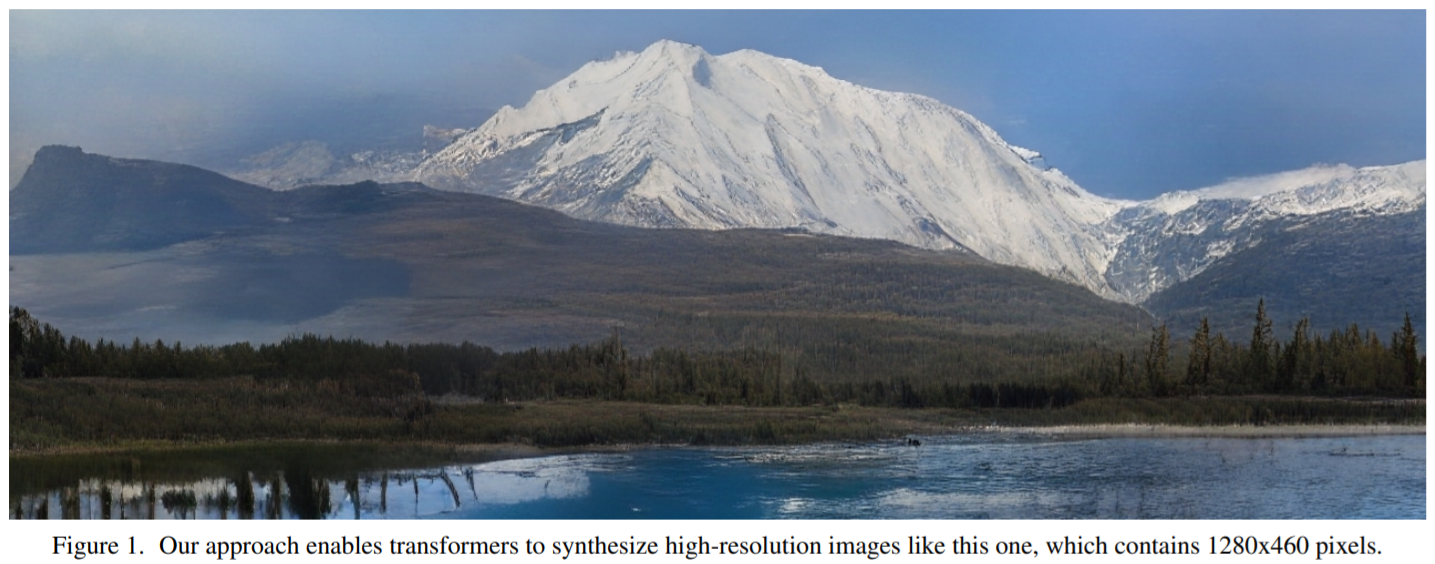
\includegraphics[width=0.7\textwidth]{img/pa5.png} 
\caption{Taming Transformers for High-Resolution Image Synthesis}
\label{Test}
\end{figure}

\subsection{Video Action Transformer Network}

本研究引入了 Action Transformer 模型,用于识别和定位视频剪辑中的人类动作,该研究重新利用了 Transformer 风格的架构,从研究中试图对其行为进行分类的人周围的时空上下文中聚合特征。研究表明,通过使用高分辨率、特定于个人、与类别无关的查询,该模型自发地学习跟踪个人并从他人的行为中获取语义上下文。此外,它的注意力机制学习强调手和脸,这对于区分动作通常是至关重要的——除了框和类别标签之外,所有这些都没有明确的监督。该研究在 Atomic Visual Actions (AVA) 数据集上训练和测试研究本身的 Action Transformer 网络,仅使用原始 RGB 帧作为输入,其性能明显优于最新技术。在此研究中,研究者的目标是定位和识别视频剪辑中的人类行为,人类行为仍然如此难以识别的一个原因是,推断一个人的行为通常需要了解周围的人和物体。比如识别一个人是否在“听某人说话”取决于场景中是否存在另一个人在说些什么。同样要识别一个人是“指着一个物体”,还是“拿着一个物体”,还是“握手”;所有这些都需要对人及其周围环境的有生命和无生命元素进行共同推理。

所以这不仅限于给定时间点的上下文而已,从识别“看人”的动作,在被看人走出画面后,需要随着时间的推移进行推理,以了解我们感兴趣的人实际上是在看人,而不仅仅是凝视远方。因此,该研究寻求一种在确定感兴趣的人的行为时可以确定和利用此类上下文信息(其他人、其他对象)的模型,Vaswani et al. 的 Transformer 架构是一个合适的模型,因为它使用自注意力明确地为其表示构建上下文支持。在此与传统的循环模型相比,这种架构在序列建模任务方面取得了巨大成功。同时另一个问题是在于,如何为人类行为识别建立一个类似的模型?其研究者的的答案是一个新的视频动作识别网络 Action Transformer,它使用修改后的 Transformer 架构作为“头部”来对感兴趣的人的动作进行分类。它汇集了另外两个想法:(i) 一个时空 I3D 模型,该模型在以前的视频动作识别方法中取得了成功,这项已提供了基本特征; (ii) 区域提议网络 (RPN) ,此项提供了一种用于定位执行动作的人的采样机制。I3D 特征和 RPN 一起生成查询,该查询是 Transformer 头的输入,该查询聚合来自周围视频中其他人和对象的上下文信息。研究者除了详细描述了这种架构也表明,经过训练的网络能够学习跟踪个人并根据视频中其他人的行为将他们的行为置于情境中。此外,转换器关注手部和面部区域,研究者已经知道它们在区分动作时具有一些最相关的特征。

所有这些都是在没有明确监督的情况下获得,而是在动作分类期间学习,并且在 Atomic Visual Actions (AVA) 数据集上训练和测试研究的模型,而对于这种上下文推理,这是一个有趣且合适的测试平台,它需要在视频中半密集地检测多个人,并识别多个基本动作。许多这些动作通常不能仅从人物边界框确定,而是需要推断与其他人和物体的关系,前者与之前的作品不同,研究者的模型无需明确的对象检测即可学会这样做。研究者在 AVA 数据集上创造了新记录,将性能从 17.4\% 提高到 25.0\% mAP。该网络仅使用原始 RGB 帧,但其性能优于之前的所有工作,包括使用额外光流和声音输入的大型集成。在提交时,该研究的方法是 ActivityNet 排行榜上表现最好的方法然而研究者也注意到在 25\% mAP 时,这个问题,甚至这个数据集,还远未解决。因此,此研究最后严格分析了模型的失败案例,该研究描述了一些常见的故障模式,并分析了按语义和空间卷标分解的性能。

同时研究者发现许多训练集相对较大的类仍然难以识别,并调查此类尾部案例以标记未来工作的潜在途径。而从图中可以知道,操作中的 Action Transformer,研究者提出的多头/层 Action Transformer 架构学习关注感兴趣的人的相关区域及其上下文(其他人、对象),以识别他们正在做的动作。每个头部计算一个剪辑嵌入,用于关注不同的部分,如面部、手和其他人,以识别感兴趣的人正在“牵手”和“看着一个人”。

\begin{figure}[htb]
\centering 
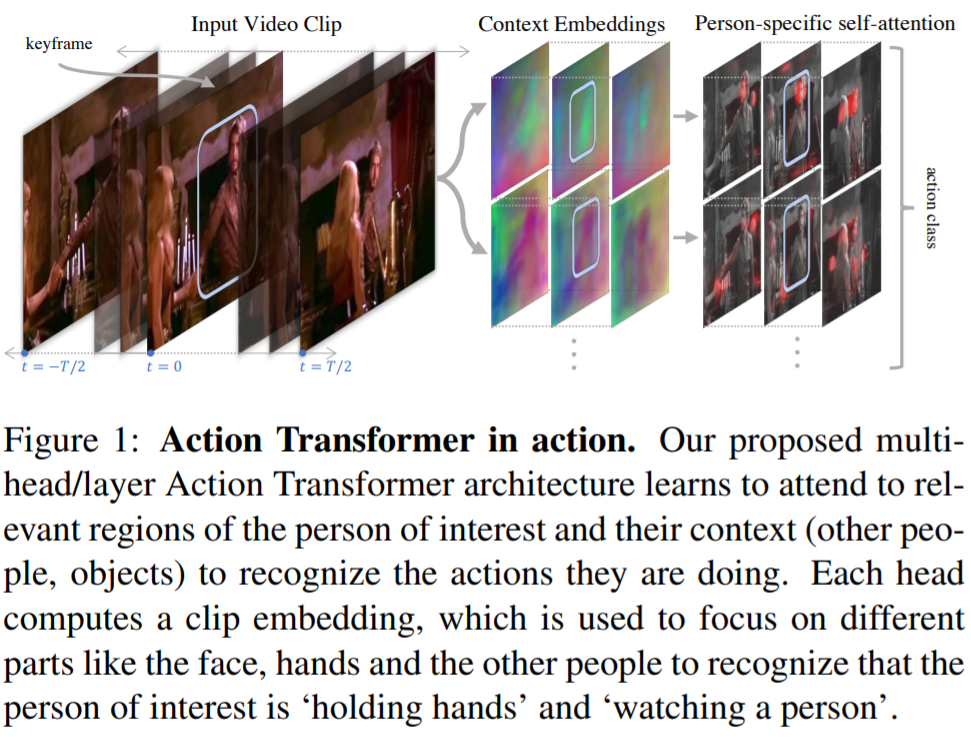
\includegraphics[width=0.7\textwidth]{img/pa6.png} 
\caption{Video Action Transformer Network}
\label{Test}
\end{figure}

\section{Transformer 工作}

该章目标在于为了呼应前述报告而对其进行复现的工作,此报告根据 Paris Dauphine University 和 Facebook AI 于 ECCV 2020 所发表的 End-to-End Object Detection with Transformers \cite{carion2020end} 进行测试。而测试的程式码则可于本专案的 code 目录中找到,其档案名称为 detr\_demo.ipynb。

\begin{figure}[htb]
\centering 
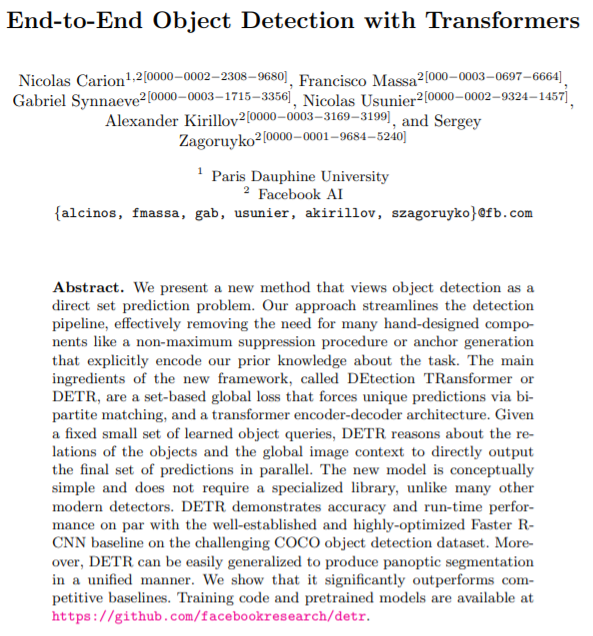
\includegraphics[width=0.7\textwidth]{img/c4d1.png} 
\caption{End-to-End Object Detection with Transformers}
\label{Test}
\end{figure}

\subsection{摘要与研究贡献}

研究者提出了一种将对象检测视为直接集预测问题的新方法,該方法简化了检测管道,並且有效地消除了对许多手工设计组件的需求,例如非最大抑制程序或锚生成,这些组件明确地编码了我们关于任务的先验知识。在此新框架的主要成分称为 DEtection TRansformer 或 DETR,其原理是基于集合的全局损失,通过二部匹配强制进行唯一预测,以及转换器编码器-解码器架构。其流程是给定一组固定的学习对象查询集,DETR 会推理对象和全局图像上下文之间的关系,以直接并行输出最终的预测集。本研究的成果与许多其他现代探测器不同,該研究的新模型在概念上很简单,不需要专门的库。而 DETR 在具有挑战性的 COCO 对象检测数据集上展示了与完善且高度优化的 Faster RCNN 基线相当的准确性和运行时性能。同時 DETR 可以很容易地推广到以统一的方式产生全景分割。

研究者先是說明对象检测的目标是为每个感兴趣的对象预测一组边界框和类别标签,而现代检测器(Modern detectors)通过在大量建议、锚点或窗口中心上定义代理回归和分类问题,以间接方式解决此集合预测任务。這些檢測器的性能受到后处理步骤的显着影响,基本上會以折叠近似重复的预测锚集的设计以及将目标框進行分配。而为了简化这些流程,我们提出了一种直接集预测方法来绕过代理任务。此類端到端的理念在复杂的结构化预测任务在如机器翻译或语音识别等方面取得了重大进展,但尚未在对象检测領域上取得重大进展與成功,而之前的尝试要么添加其他形式的先验知识 ,或者没有被证明在具有挑战性的基准上具有强大的基线竞争力。而本研究的目標就是想要弥合这一個差距,其研究者通过将对象检测视为直接集预测问题来简化训练管道。他們采用基于转换器 的编码器-解码器架构,这是一种流行的序列预测架构。

转换器的自注意力机制显式地对序列中元素之间的所有成对交互进行建模,使这些架构特别适用于集合预测的特定约束,例如删除重复预测。該研究的检测变换器 DETR  會一次预测所有对象,并使用一组损失函数进行端到端训练,该函数在预测对象和真实对象之间执行二分匹配。而所謂的 DETR 會通过将常见的 CNN 与变压器架构相结合,直接预测(并行)最终检测集,在模型進行训练期间,二分匹配使用真实值框唯一地進行分配预测,而没有匹配的预测应产生“无对象”(∅)类的预测。DETR 通过删除多个手工设计的编码先验知识的组件来简化检测管道,如空间锚点或非最大抑制。而 DETR 与大多数现有检测方法不同,DETR 本身不需要任何自定义层,因此可以在包含标准 ResNet 和 Transformer 类的任何框架中轻松重现。該模型与之前关于直接集预测的大多数工作相比,DETR 的主要特征是二部匹配损失和变换器与非自回归的并行解码的结合。跟過往的研究相較之下,其工作侧重于使用 RNN 进行自回归解码。而研究者的匹配损失函数唯一地将预测分配给真实对象,并且对预测对象的排列是不变的,因此該研究可以并行发出它们。

最後研究團隊在最流行的对象检测数据集 COCO 上评估 DETR,將 DETR 與非常有竞争力的 Faster R-CNN 基线相比,Faster RCNN 经历了多次设计迭代,其性能自最初发布以来得到了极大的提升。研究的实验表明,其研究的新模型实现了可比的性能,DETR 在大型对象上表现出明显更好的性能,这一结果可能是由转换器的非本地计算实现的。然而 DETR 在小物体上的性能较低,研究者预计未来的工作将以与 FPN 为 Faster R-CNN 所做的开发相同的方式改进这方面,同時 DETR 的训练设置与标准物体检测器有多种不同。而新模型需要超长的训练计划,并受益于变压器中的辅助解码损失,同時該研究也徹底探索了哪些组件对展示的性能是至关重要部分,而且 DETR 的设计理念很容易扩展到更复杂的任务。=在研究者的实验中表明在预训练的 DETR 之上训练的简单分割头优于全景分割的竞争基线,这是一项近期具有挑战性的像素级识别任务。

\subsection{程式码与演示}

在此根据专案的论文测试的程式码进行呈现,而该档案则可于本专案的 code 目录中找到,其档案名称为 detr\_demo.ipynb。而在此使用 DETR 进行对象检测,研究者展示了名为 DETR 检测变换器的演示并展示了如何定义模型、加载预训练权重以及可视化边界框和类别预测。

1. 套件与环境

\begin{Verbatim}
from PIL import Image
import requests
import matplotlib.pyplot as plt
%config InlineBackend.figure_format = 'retina'

import torch
from torch import nn
from torchvision.models import resnet50
import torchvision.transforms as T
torch.set_grad_enabled(False);
\end{Verbatim}

2. DETR 实现

\begin{Verbatim}
class DETRdemo(nn.Module):
    """
    Demo DETR implementation.

    Demo implementation of DETR in minimal number of lines, with the
    following differences wrt DETR in the paper:
    * learned positional encoding (instead of sine)
    * positional encoding is passed at input (instead of attention)
    * fc bbox predictor (instead of MLP)
    The model achieves ~40 AP on COCO val5k and runs at ~28 FPS on Tesla V100.
    Only batch size 1 supported.
    """
    def __init__(self, num_classes, hidden_dim=256, nheads=8,
                 num_encoder_layers=6, num_decoder_layers=6):
        super().__init__()

        # create ResNet-50 backbone
        self.backbone = resnet50()
        del self.backbone.fc

        # create conversion layer
        self.conv = nn.Conv2d(2048, hidden_dim, 1)

        # create a default PyTorch transformer
        self.transformer = nn.Transformer(
            hidden_dim, nheads, num_encoder_layers, num_decoder_layers)

        # prediction heads, one extra class for predicting non-empty slots
        # note that in baseline DETR linear_bbox layer is 3-layer MLP
        self.linear_class = nn.Linear(hidden_dim, num_classes + 1)
        self.linear_bbox = nn.Linear(hidden_dim, 4)

        # output positional encodings (object queries)
        self.query_pos = nn.Parameter(torch.rand(100, hidden_dim))

        # spatial positional encodings
        # note that in baseline DETR we use sine positional encodings
        self.row_embed = nn.Parameter(torch.rand(50, hidden_dim // 2))
        self.col_embed = nn.Parameter(torch.rand(50, hidden_dim // 2))

    def forward(self, inputs):
        # propagate inputs through ResNet-50 up to avg-pool layer
        x = self.backbone.conv1(inputs)
        x = self.backbone.bn1(x)
        x = self.backbone.relu(x)
        x = self.backbone.maxpool(x)

        x = self.backbone.layer1(x)
        x = self.backbone.layer2(x)
        x = self.backbone.layer3(x)
        x = self.backbone.layer4(x)

        # convert from 2048 to 256 feature planes for the transformer
        h = self.conv(x)

        # construct positional encodings
        H, W = h.shape[-2:]
        pos = torch.cat([
            self.col_embed[:W].unsqueeze(0).repeat(H, 1, 1),
            self.row_embed[:H].unsqueeze(1).repeat(1, W, 1),
        ], dim=-1).flatten(0, 1).unsqueeze(1)

        # propagate through the transformer
        h = self.transformer(pos + 0.1 * h.flatten(2).permute(2, 0, 1),
                             self.query_pos.unsqueeze(1)).transpose(0, 1)
        
        # finally project transformer outputs to class labels and bounding boxes
        return {'pred_logits': self.linear_class(h), 
                'pred_boxes': self.linear_bbox(h).sigmoid()}
\end{Verbatim}


由于 Transformer 的表示能力,DETR 架构非常简单。 有两个主要组成部分:

\begin{itemize}
\item [1.] 一个卷积主干——我们在这个演示中使用 ResNet-50
\item [2.] 一个 Transformer - 我们使用默认的 PyTorch nn.Transformer
\end{itemize}

\begin{figure}[htb]
\centering 
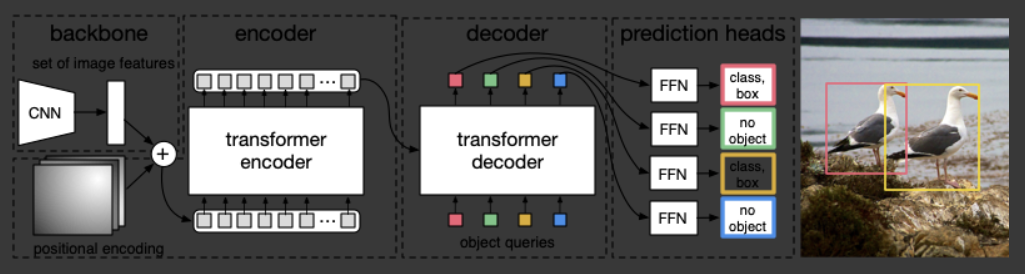
\includegraphics[width=0.7\textwidth]{img/c4d2.png} 
\caption{DETR 架构}
\label{Test}
\end{figure}

让我们用 80 个 COCO 输出类 + 1 $\emptyset$ “无对象”类构建模型并加载预训练的权重。 权重以半精度保存,以节省带宽而不影响模型精度。

3. 载入训练

\begin{Verbatim}
detr = DETRdemo(num_classes=91)
state_dict = torch.hub.load_state_dict_from_url(
    url='https://dl.fbaipublicfiles.com/detr/detr_demo-da2a99e9.pth',
    map_location='cpu', check_hash=True)
detr.load_state_dict(state_dict)
detr.eval();
\end{Verbatim}

4. 使用 DETR 计算预测

加载的预训练 DETR 模型已经在 80 个 COCO 类上进行了训练,类索引从 1 到 90(这就是我们在模型构建中考虑 91 个类的原因)。 在以下单元格中,我们定义了从类索引到名称的映射。

\begin{Verbatim}
# COCO classes
CLASSES = [
    'N/A', 'person', 'bicycle', 'car', 'motorcycle', 'airplane', 'bus',
    'train', 'truck', 'boat', 'traffic light', 'fire hydrant', 'N/A',
    'stop sign', 'parking meter', 'bench', 'bird', 'cat', 'dog', 'horse',
    'sheep', 'cow', 'elephant', 'bear', 'zebra', 'giraffe', 'N/A', 'backpack',
    'umbrella', 'N/A', 'N/A', 'handbag', 'tie', 'suitcase', 'frisbee', 'skis',
    'snowboard', 'sports ball', 'kite', 'baseball bat', 'baseball glove',
    'skateboard', 'surfboard', 'tennis racket', 'bottle', 'N/A', 'wine glass',
    'cup', 'fork', 'knife', 'spoon', 'bowl', 'banana', 'apple', 'sandwich',
    'orange', 'broccoli', 'carrot', 'hot dog', 'pizza', 'donut', 'cake',
    'chair', 'couch', 'potted plant', 'bed', 'N/A', 'dining table', 'N/A',
    'N/A', 'toilet', 'N/A', 'tv', 'laptop', 'mouse', 'remote', 'keyboard',
    'cell phone', 'microwave', 'oven', 'toaster', 'sink', 'refrigerator', 'N/A',
    'book', 'clock', 'vase', 'scissors', 'teddy bear', 'hair drier',
    'toothbrush'
]

# colors for visualization
COLORS = [[0.000, 0.447, 0.741], [0.850, 0.325, 0.098], [0.929, 0.694, 0.125],
          [0.494, 0.184, 0.556], [0.466, 0.674, 0.188], [0.301, 0.745, 0.933]]
\end{Verbatim}


DETR 使用标准的 ImageNet 归一化,并以 $[x_{\text{center}}, y_{\text{center}}, w, h]$ 格式输出相对图像坐标中的框,其中 $[x_{\text{center}}, y_{\text{center}}]$ 是边界框的预测中心,$w, h$ 是其宽度和高度。 因为坐标是相对于图像尺寸的,并且位于 $[0, 1]$ 之间,我们将预测转换为绝对图像坐标和 $[x_0, y_0, x_1, y_1]$ 格式以用于可视化目的。

\begin{Verbatim}
# standard PyTorch mean-std input image normalization
transform = T.Compose([
    T.Resize(800),
    T.ToTensor(),
    T.Normalize([0.485, 0.456, 0.406], [0.229, 0.224, 0.225])
])

# for output bounding box post-processing
def box_cxcywh_to_xyxy(x):
    x_c, y_c, w, h = x.unbind(1)
    b = [(x_c - 0.5 * w), (y_c - 0.5 * h),
         (x_c + 0.5 * w), (y_c + 0.5 * h)]
    return torch.stack(b, dim=1)

def rescale_bboxes(out_bbox, size):
    img_w, img_h = size
    b = box_cxcywh_to_xyxy(out_bbox)
    b = b * torch.tensor([img_w, img_h, img_w, img_h], dtype=torch.float32)
    return b
\end{Verbatim}

把所有东西放在一个检测函数中:

\begin{Verbatim}
def detect(im, model, transform):
    # mean-std normalize the input image (batch-size: 1)
    img = transform(im).unsqueeze(0)

    # demo model only support by default images with aspect ratio between 0.5 and 2
    # if you want to use images with an aspect ratio outside this range
    # rescale your image so that the maximum size is at most 1333 for best results
    assert img.shape[-2] <= 1600 and img.shape[-1] <= 1600, 'demo model'

    # propagate through the model
    outputs = model(img)

    # keep only predictions with 0.7+ confidence
    probas = outputs['pred_logits'].softmax(-1)[0, :, :-1]
    keep = probas.max(-1).values > 0.7

    # convert boxes from [0; 1] to image scales
    bboxes_scaled = rescale_bboxes(outputs['pred_boxes'][0, keep], im.size)
    return probas[keep], bboxes_scaled
\end{Verbatim}

5. 使用 DETR

在此使用本作业专案的图进行测试,从网路上任意抓得仓鼠、考拉、柯基犬与范例的猫。

\begin{figure}[htb]
  \centering
  \subfloat[測試 - 仓鼠]{
    \label{Fig.sub.1}
    
\includegraphics[width=0.3\textwidth]{img/r1.jpg}}
  \subfloat[測試 - 考拉]{
    \label{Fig.sub.2}
    
\includegraphics[width=0.3\textwidth]{img/r2.jpg}}
  \subfloat[測試 - 柯基犬]{
    \label{Fig.sub.1}
    %
\includegraphics[height=2cm]{img/r3.jpg}}
    
\includegraphics[width=0.3\textwidth]{img/r3.jpg}}
  \caption{最终自有测试资料集}
  \label{Fig.main}
\end{figure}

6. 结果输出

在此可以观察到加入的仓鼠并没有被辨识出来,同时研究中所用的猫能够被正确辨识之外,柯基犬被辨识成狗,而考拉则被辨识成熊。

\begin{Verbatim}
def plot_results(pil_img, prob, boxes):
    plt.figure(figsize=(16,10))
    plt.imshow(pil_img)
    ax = plt.gca()
    for p, (xmin, ymin, xmax, ymax), c in zip(prob, boxes.tolist(), COLORS * 100):
        ax.add_patch(plt.Rectangle((xmin, ymin), xmax - xmin, ymax - ymin,
                                   fill=False, color=c, linewidth=3))
        cl = p.argmax()
        text = f'{CLASSES[cl]}: {p[cl]:0.2f}'
        ax.text(xmin, ymin, text, fontsize=15,
                bbox=dict(facecolor='yellow', alpha=0.5))
    plt.axis('off')
    plt.show()
    
plot_results(im1, scores1, boxes1)
plot_results(im2, scores2, boxes2)
plot_results(im3, scores3, boxes3)
plot_results(im4, scores4, boxes4)
\end{Verbatim}

\begin{figure}[htb]
\centering 
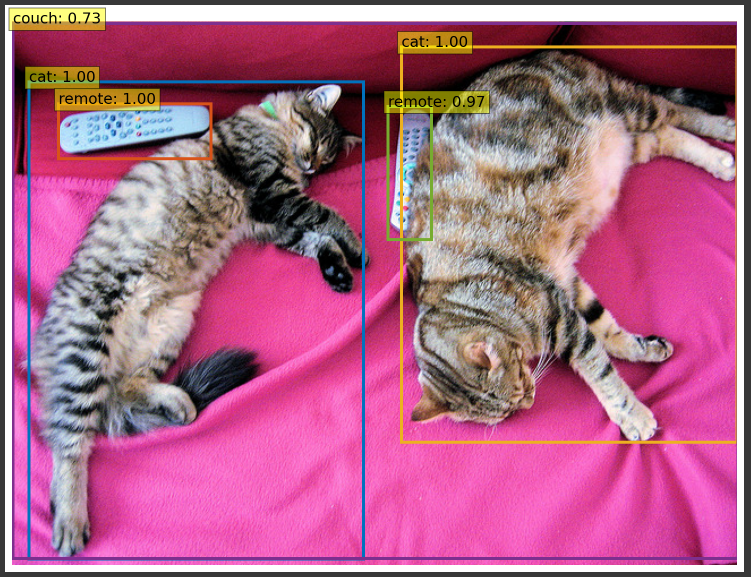
\includegraphics[width=0.85\textwidth]{img/c4d3.png} 
\caption{测试 - 猫}
\label{Test}
\end{figure}

\begin{figure}[htb]
\centering 
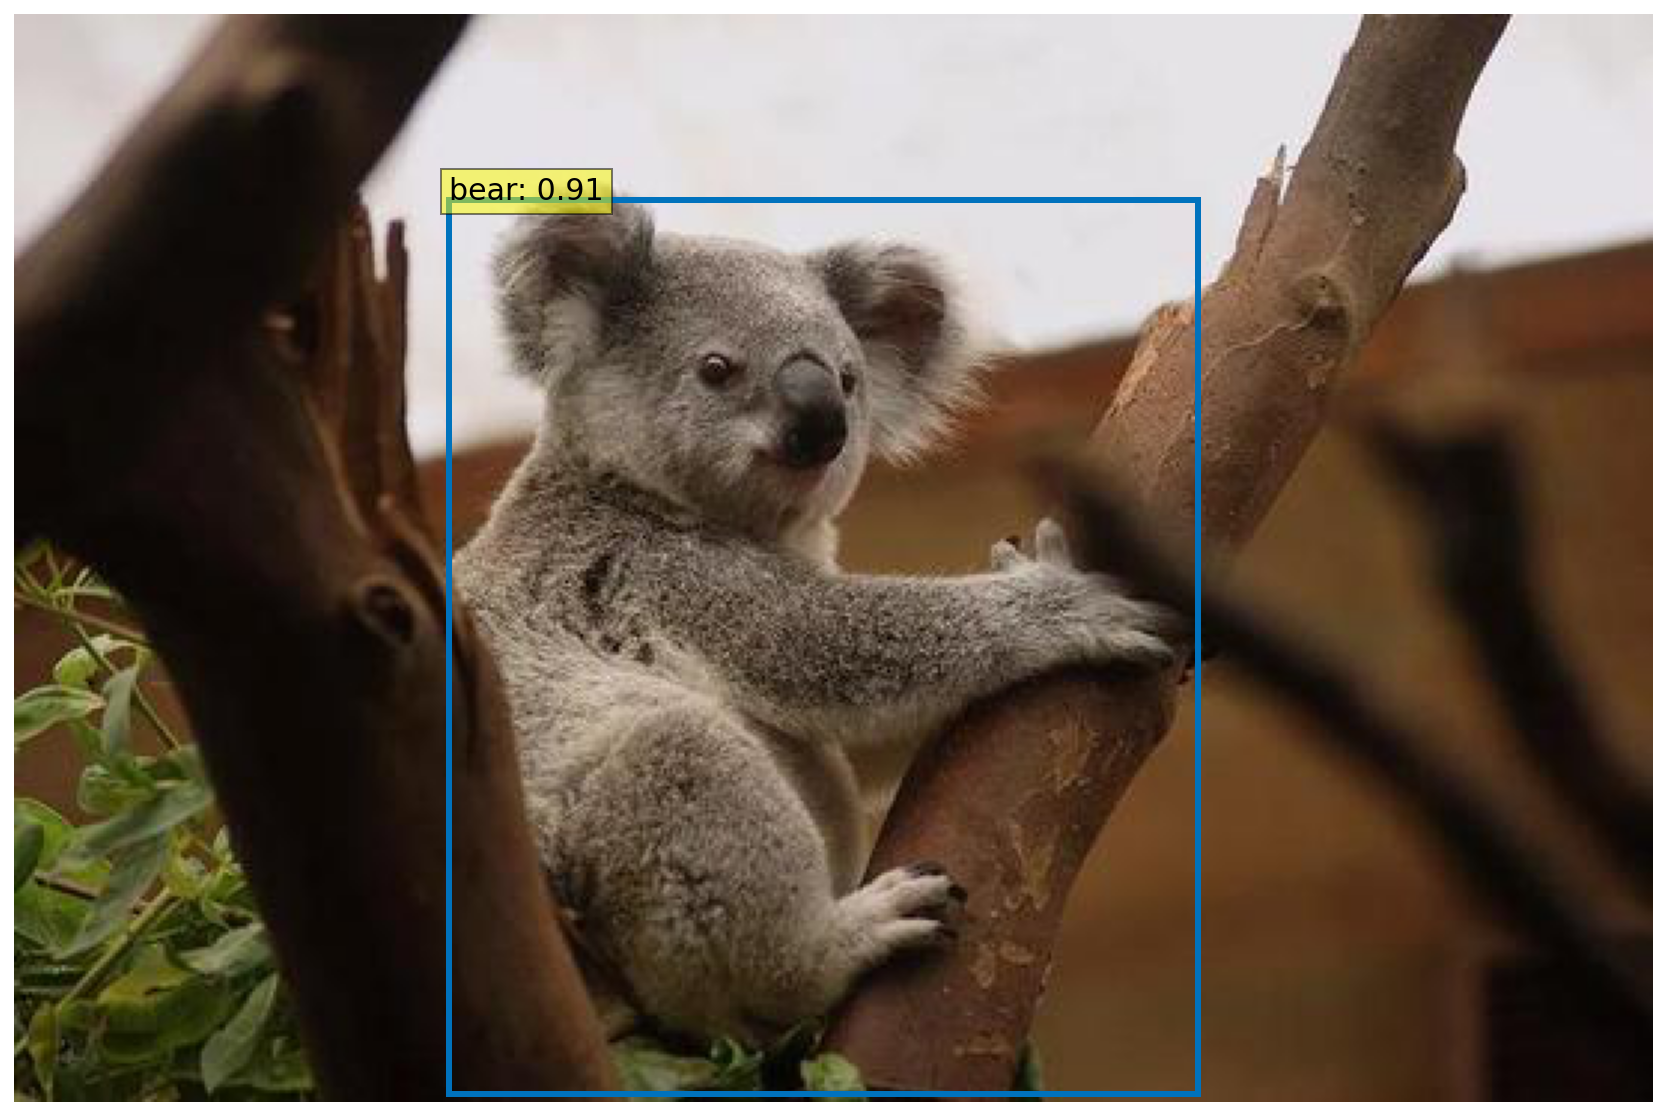
\includegraphics[width=0.85\textwidth]{img/c4d4.png} 
\caption{测试 - 考拉}
\label{Test}
\end{figure}

\begin{figure}[htb]
\centering 
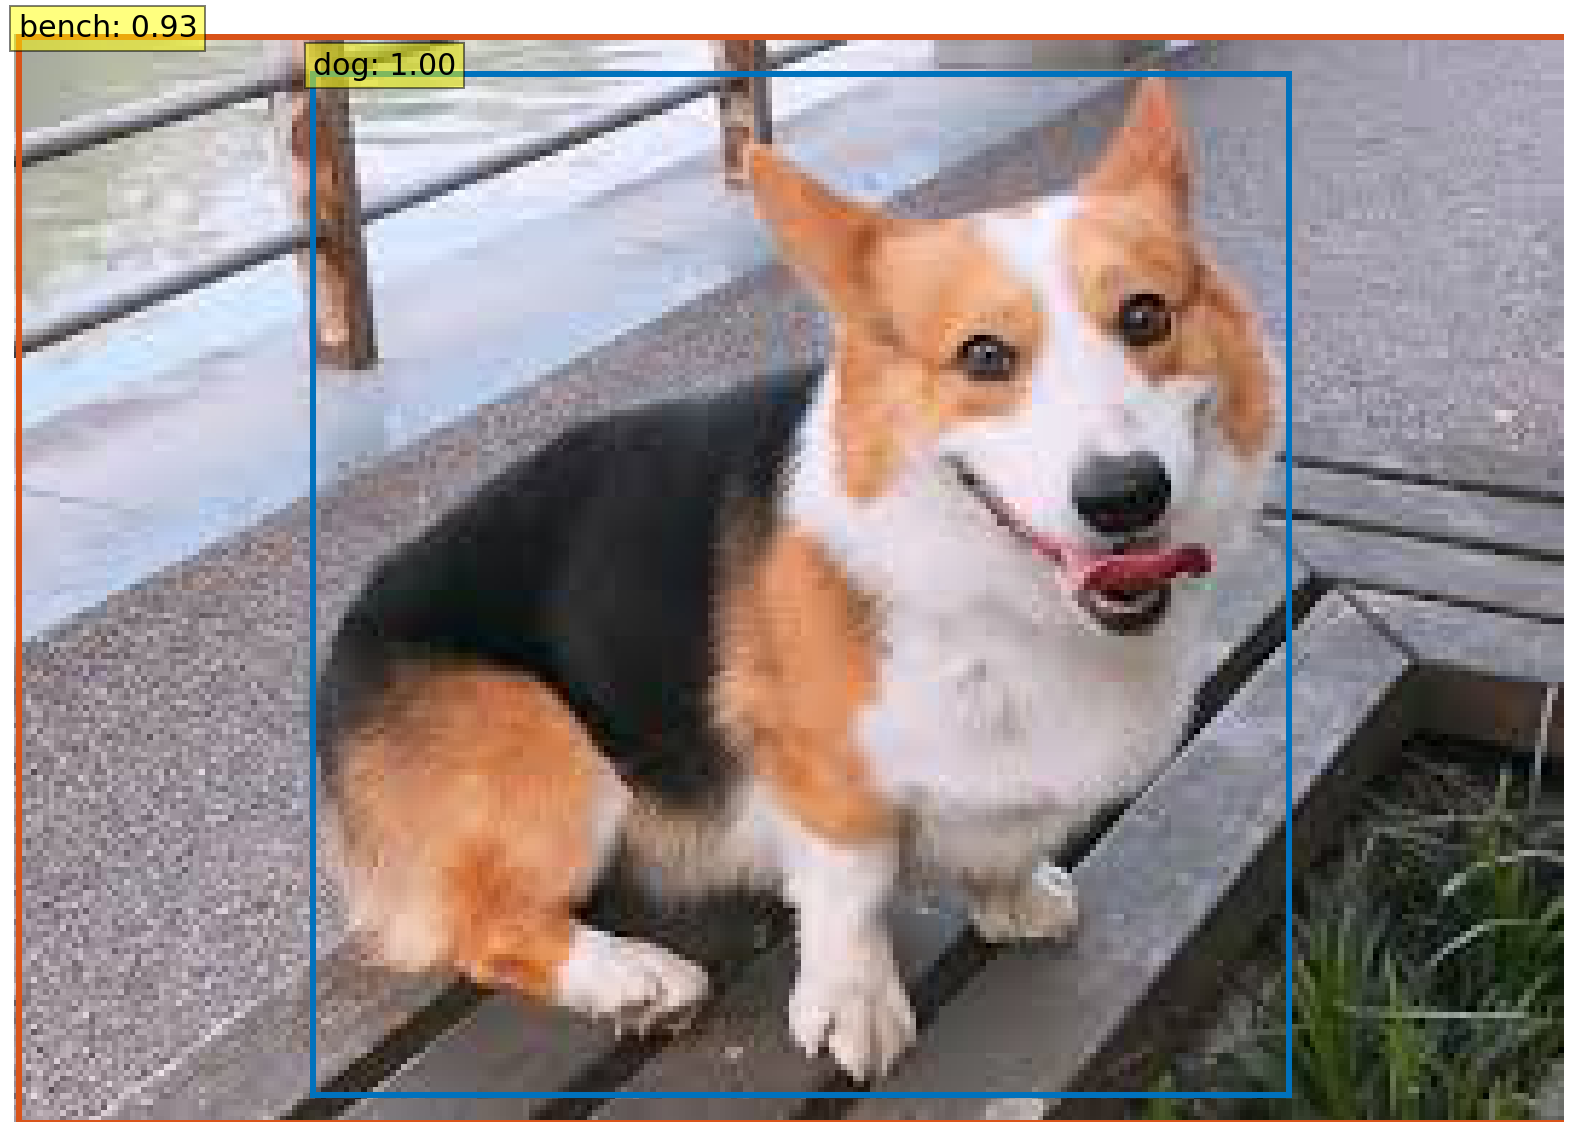
\includegraphics[width=0.85\textwidth]{img/c4d5.png} 
\caption{测试 - 柯基}
\label{Test}
\end{figure}